% -----------------------------------------------------
% QUESTION
% -----------------------------------------------------
\question[20]
\textbf{Desafío:} Dado $a\geq{0}$, calcule el siguiente límite:
$$\lim_{x \to 0} \frac{a^x-a^{\sin{x}}}{x^3}$$
Pista (1): Recuerda sacar las constantes del límite (opcional).\\
Pista (2): Si vas a la mitad del ejercicio y no te preguntas “cómo es posible”, hazlo de nuevo.\\
Pista (3): La dificultad del ejercicio es solamente lo largo, si vas determinado es relativamente fácil!
% -----------------------------------------------------
\mostrarpuntaje

\begin{solution}
    \begin{center}
        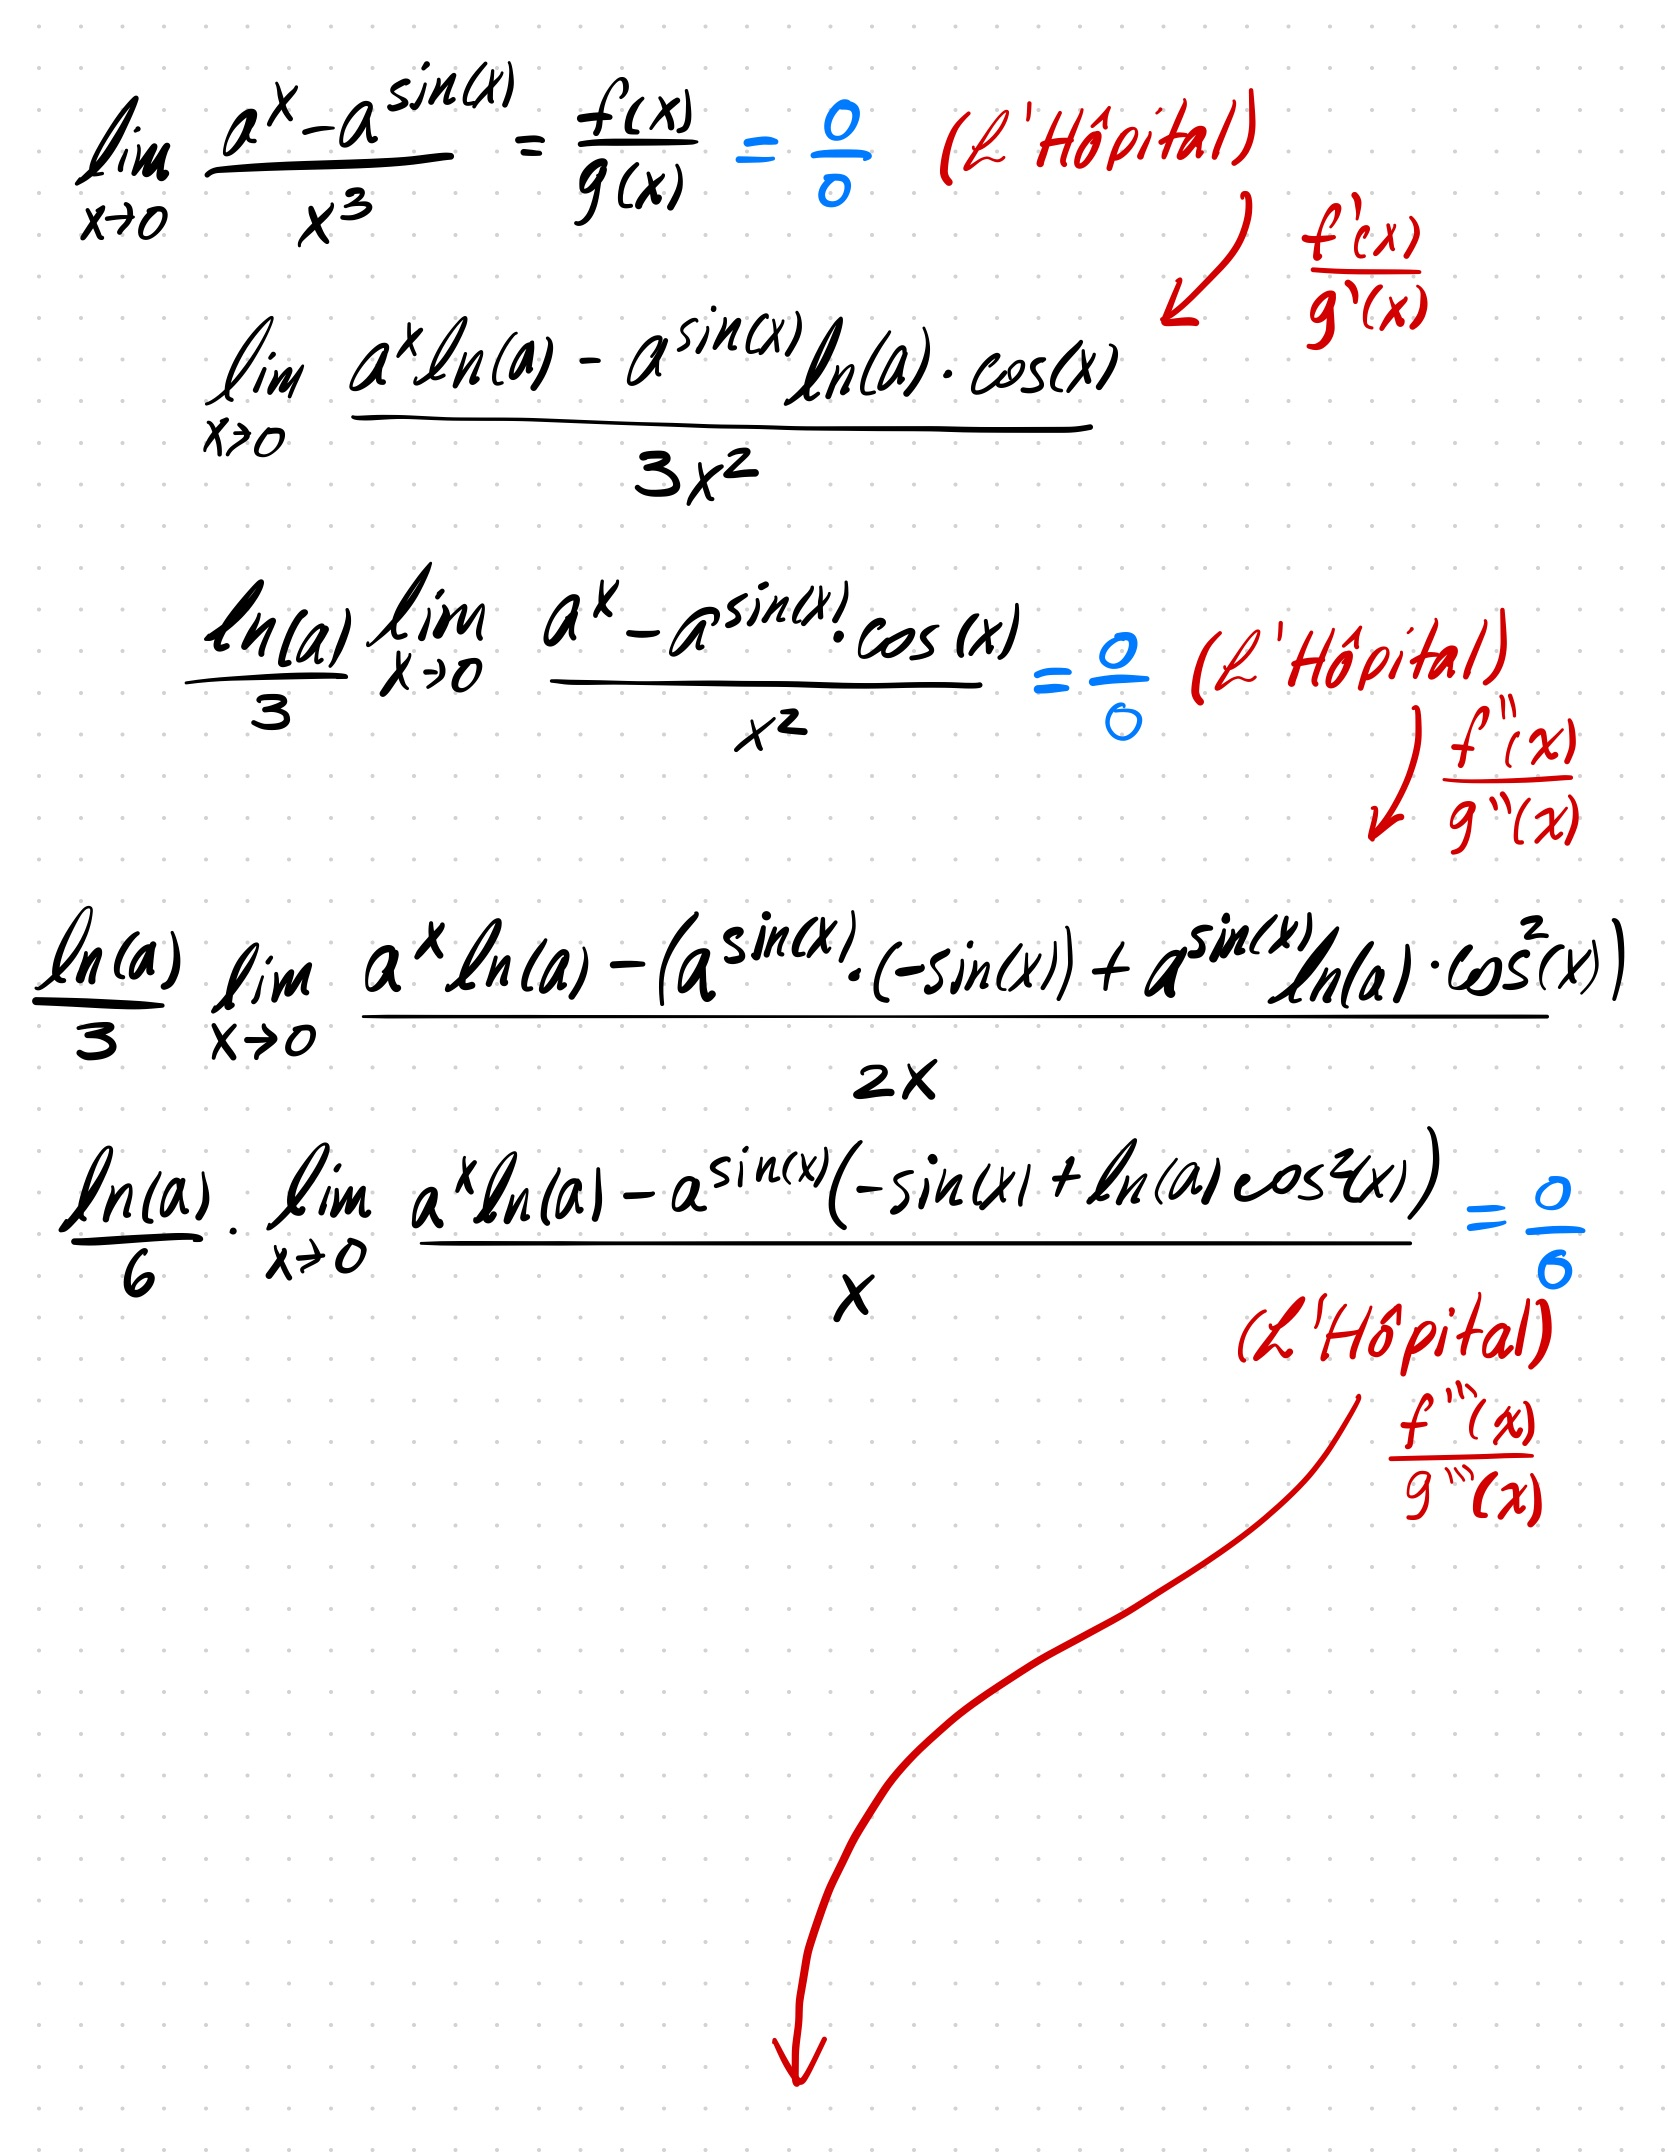
\includegraphics[width=0.7\linewidth]{des1.jpg}
    \end{center}
    \begin{center}
        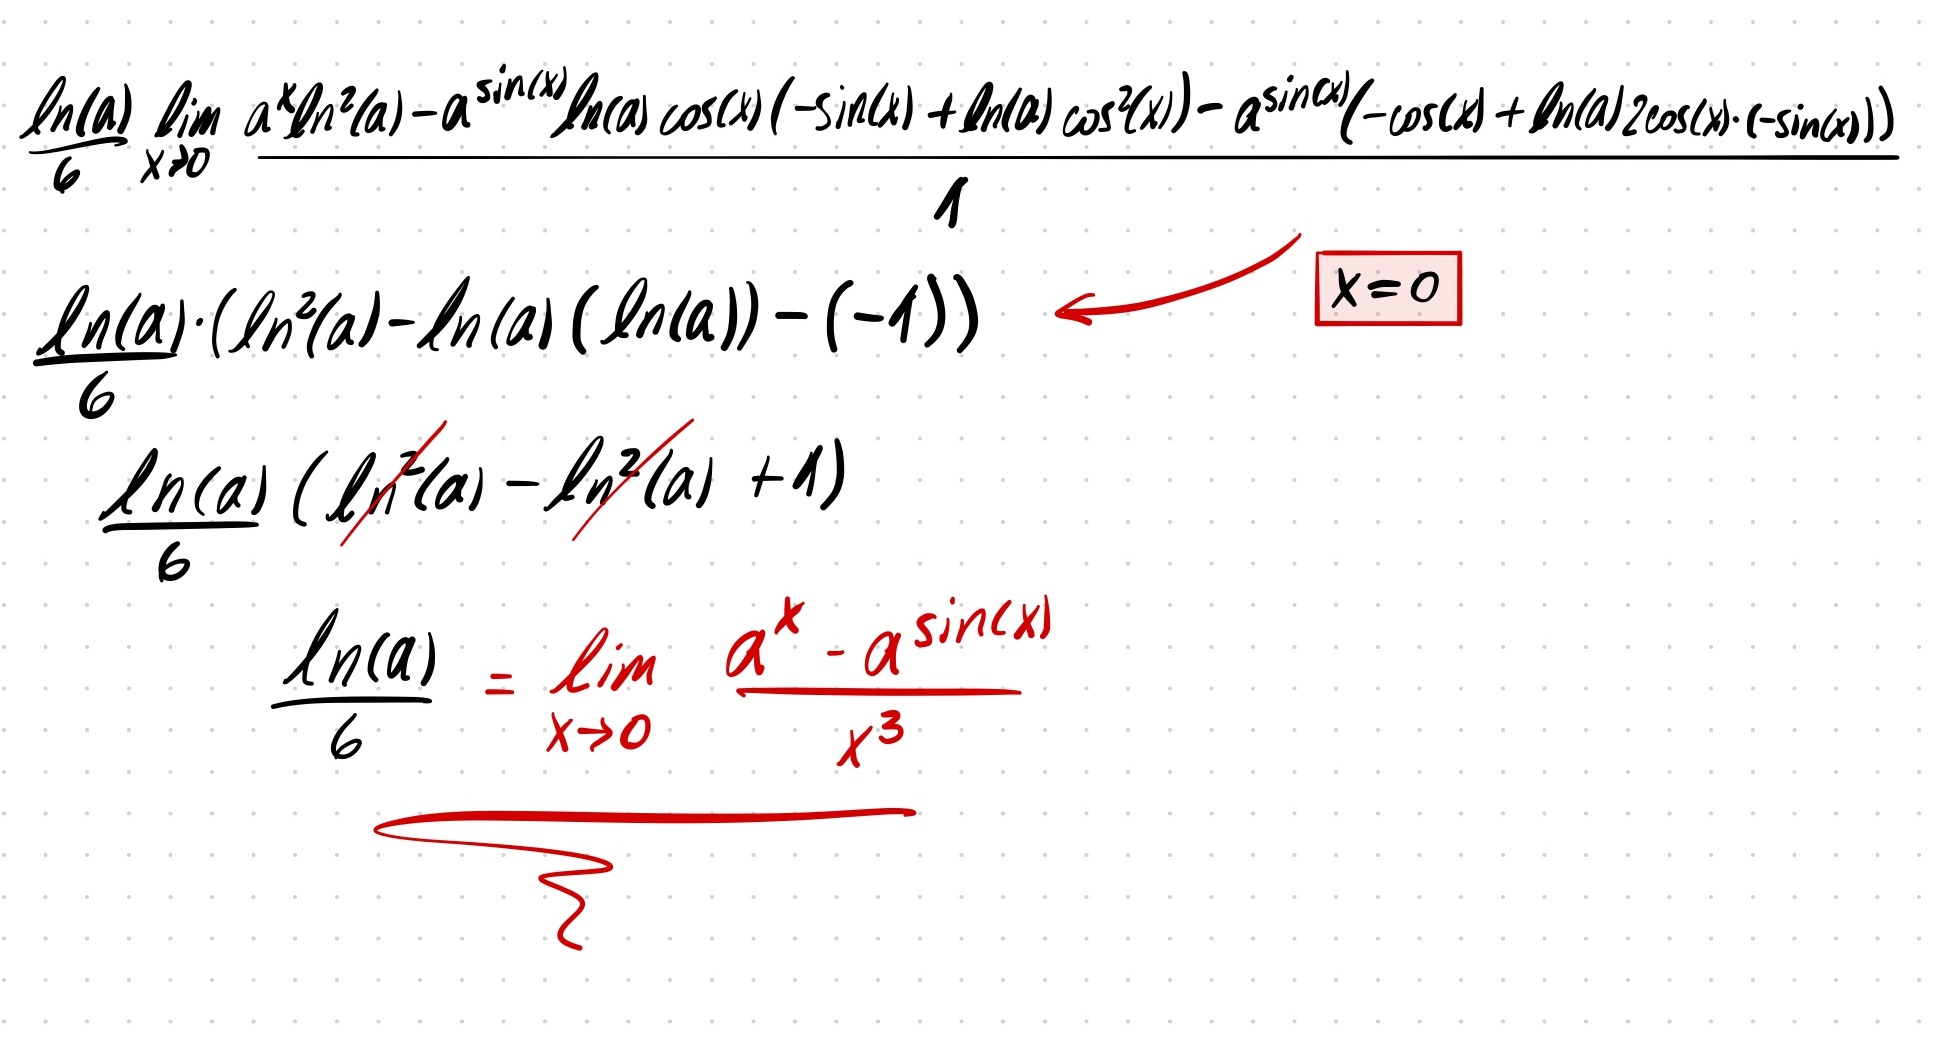
\includegraphics[width=\linewidth]{des2.jpg}
    \end{center}
\end{solution}
